\begin{figure}[t]\centering
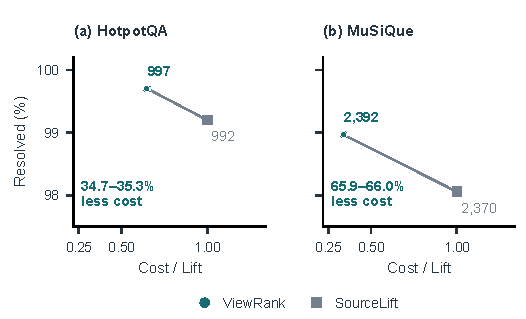
\includegraphics[width=\columnwidth]{../figures/domain_performance.pdf}
\caption{Complete cost and resolution in layout-matched cohort A at 16\,MiB: 1,000/2,417 HotpotQA/MuSiQue questions. Cost is divided by paired compressed SourceLift; all three blocks are plotted and can overlap. Lines join median operating points. Counts require all three cutoffs resolved (\stable\ or verified \unstable); the labeled vertical range magnifies the small coverage differences. All requests, including \unknown, remain charged.}
\label{fig:domain-performance}
\end{figure}
Figure~\ref{fig:domain-performance} places the strongest layout-matched comparison in the cost--resolution plane: ViewRank moves toward lower complete cost and more resolved audits on both workloads. Figure~\ref{fig:domain-coupling} locates the largest active-cost gains in the coupled-source work addressed by the compiler. Table~\ref{tab:domain-main} separately retains the competitive DensePruned layouts and the original full-response controls.

\begin{figure}[t]\centering
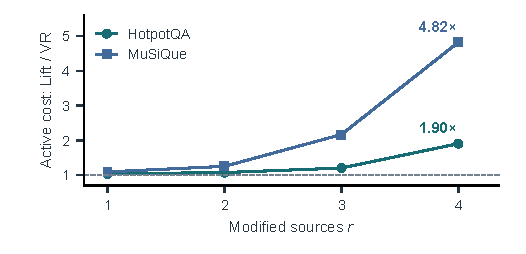
\includegraphics[width=\columnwidth]{../figures/domain_coupling.pdf}
\caption{Source-count strata in cohort A. Lines join medians of three paired ratios of summed active cost; dots retain every block. Every stratum includes \unknown\ requests. Startup/setup are excluded here. Repeated blocks are descriptive, not confidence intervals.}
\label{fig:domain-coupling}\end{figure}
